\textbf{Consider the predictor-corrector time-stepping scheme:}
\begin{align*}
& y_{n+1}^p = y_n + \frac{\Delta t}{12}(23f_n - 16f_{n-1}+5f_{n-2}), \\
&y_{n+1} = y_n + \frac{\Delta t}{12}(5f(t_{n+1},y_{n+1}^p) + 8f)n - f_{n-1})~.
\end{align*}
\textbf{where $f_n = f(t_n,y_n)$ and $y'(t) = f(t,y)$, $y(0) = y_0$. Plot the stability region for this scheme.}

Let $f_n = \lambda y^{n}$ and $a = \frac{\Delta t \lambda}{12}$. We start by simply substituting $y_{n+1}^p$ from the first equation into the second,
\begin{align*}
y^{n+1} = y^n + a \left[ 5(y^n + a(23y^n- 16y^{n-1}+5y^{n-1})) + 8y^n - y^{n-1} \right]~.
\end{align*} 
Further let $y^{n+1} = gy^n$,
\begin{align*}
gy^n = y^n +a\left[ 5y^n + 115ay^n - 80\frac{a}{g}y^n + 25\frac{a}{g^2}y^n\right] + 8ay^n - \frac{a}{g}y^n.
\end{align*}
Reorganizing the terms, we obtain a second degree polynomial for $a$,
\begin{align*}
(115g^2 - 80g +25)a^2 + (13g^2-g)a + (g^2-g^3) = 0,
\end{align*}
which gives us the solution
\begin{align*}
a = \frac{-(13g^2 - g) \pm \sqrt{(13g^2-g)^2 - 4(115g^2 - 80g+25)(g^2-g^3)}}{2(115g^2 - 80g +25)}.
\end{align*}
Note that $z =\Delta t\lambda= 12a$, 
\begin{align*}
z =12 \frac{-(13g^2 - g) \pm \sqrt{(13g^2-g)^2 - 4(115g^2 - 80g+25)(g^2-g^3)}}{2(115g^2 - 80g +25)}.
\end{align*}
We plot the previos in \textsl{Matlab} and obatin stability region shown in the next figure.

\begin{figure}[H]
\centering     %%% not \center
{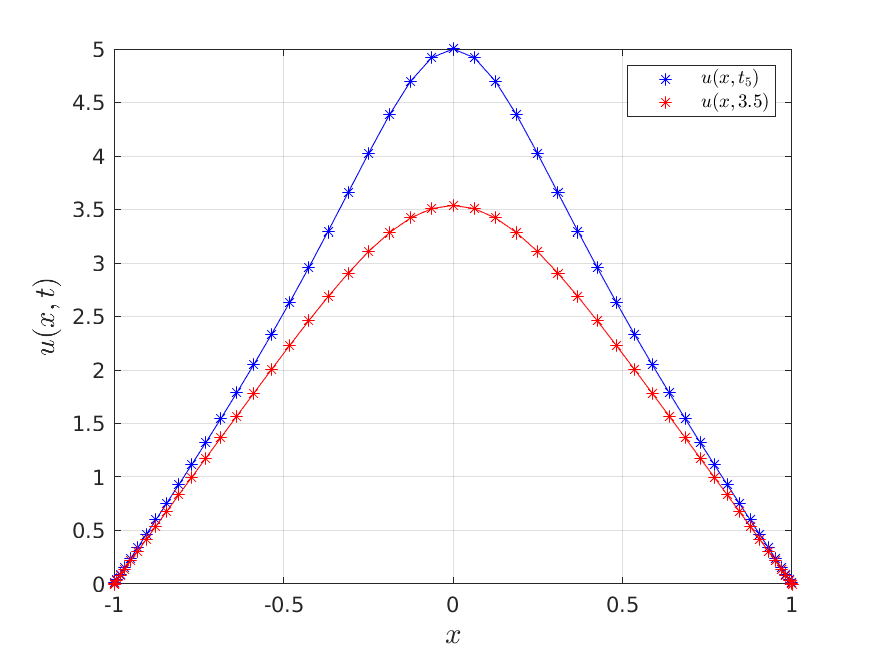
\includegraphics[scale=0.75]{P3.eps}}
\caption{Stability region.}
\end{figure}

\subsection*{Matlab code for this problem}
\begin{verbatim}
%% Problem 3
clear variables
close all
clc
N=300;
theta = linspace(0,2*pi,N);
g=exp(1i*theta);
a=115*g.^2-80*g+25;
b=13*g.^2-g;
c=g.^2-g.^3;
sq=sqrt(b.^2-4*a.*c);
zp=12*(-b+sq)./(2*a);
zn=12*(-b-sq)./(2*a);
figure
plot(real(zp),imag(zp),'b.')
hold on
plot(real(zn),imag(zn),'b.')
grid on
axis('image', [-2.5 0.5 -1.5 1.5])
xlabel('$\Re(z)$','interpreter','latex'...
    ,'fontsize',16)
ylabel('$\Im(z)$','interpreter','latex'...
    ,'fontsize',16)
txt='Latex/FIGURES/P3';
saveas(gcf,txt,'epsc')
\end{verbatim}